\section{Introducción}
La creación del \hyperlink{abbr}{SDAC} fue un proceso si bien directo de la
propuesta al sistema, largo gracias a la complejidad computacional del modelo
que realizará la inferencia. Como se expuso, previamente los sistemas de apoyo
al diagnóstico eran caros y poco presentes dentro del laboratorio; al crear un
sistema diseñado desde el concepto para maximizar su presencia y su uso por el
experto, se asegura que pueda reducir las muertes por \hyperlink{abbr}{CCU} en
nuestro país gracias a la detección rápida y temprana de las lesiones
morfológicas que lo originan. 

Concluimos esta tesis presentando un condensado de los resultados de los
experimentos realizados, una reseña del trabajo a futuro necesario para
convertir la solución en un sistema y cerramos con unas conclusiones pertinentes
y algunos comentarios del desarrollo completo de la tesis.


\section{Planteamiento del problema}
% Creo que ya quedó el planteamiento :D
El \hyperlink{abbr}{CCU} es uno de los dos tipos de cáncer ubicuos al sexo
femenino. Siendo, por su grado de mortandad en comparación a todos los demás
tipos, el segundo de mayor importancia. A nivel global,  el 12\% de todos los
cánceres femeninos son
CCU.~\cite{CancerToday-InstitutionalAgencyforResearchonCancerWHO2018}

Aparte de la tasa de mortandad, el \hyperlink{abbr}{CCU} resulta ser un factor
de alto impacto social por varias circunstancias. La primera es que, por la
naturaleza del tratamiento, la persona queda inhabilitada por la agresividad del
mismo; en familias de escasos recursos, donde la probabilidad de perecer de
cáncer es más alta y donde en varias ocasiones la madre es la única que trae
sustento al hogar. En segundo lugar, si la persona cuenta con acceso a salud
pública, tratar y curar el cáncer conlleva en una gran carga económica para el
Estado y para los contribuyentes; si la persona se decide por la salud privada,
el costo de la misma fácilmente puede hacer que baje una o varias clases
económicas.~\cite{SecretariadeSalud2015a}

La única manera para reducir estos impactos es mediante un diagnóstico rápido y
temprano del cáncer: la tasa de supervivencia es directamente proporcional a que
tan temprano se haga el diagnóstico y el cáncer en etapas tempranas,
lógicamente, es más rápido y menos costoso de curar.~\cite{WorldHealthOrganization}

Este diagnóstico se realiza mediante el análisis visual de las muestras tomadas
por el examen de Papanicolau. Dicho examen, al ser considerado de rutina y con
carácter crucial en los hospitales genera un volumen de pruebas bastante
elevado, lo que conlleva a una reducción en la eficacia de diagnóstico que puede
costar vidas e incide directamente en la precisión. La eficacia se reduce debido
a que muchas veces los hospitales o clínicas carecen del personal necesario para
analizar todas las muestras, por ejemplo, un laboratorio consultado de patología
recibe un número de muestras ronda las 500 unidades diarias, lo cual resulta
excesivo para las personas que trabajan en dicho
laboratorio.~\cite{DelMoral2017} 

Las pruebas manuales de \hyperlink{abbr}{PAP} son un reto debido a que es un
trabajo repetitivo, intensivo, tiene alta incidencia de falsos positivos y
negativos, conlleva riesgo ergonómico y puede ser afectado significativamente
por el ambiente en el cual se tomó la muestra. Esta dificultad aparte se ve
exacerbada por la falta de cito-tecnólogos.~\cite{Cucoranu2014}

La precisión se reduce cuando una persona tiene que analizar demasiadas muestras
y por fatiga ocular o mental, comienza a generar errores en el diagnóstico, es
común que una persona que se dedique a realizar el diagnóstico realice horas
extras y tenga sobrecarga de trabajo. Otro factor que afecta en la eficacia del
diagnóstico, es que cada experto tiene su propia heurística mental al
diagnosticar casos limítrofes, esto genera subjetividad y falta de consenso
médico en el diagnóstico con lo cual se genera lentitud en el mismo. Todo esto
compone la problemática técnica. Los especialistas, requieren herramientas que
los asistan en la realización de su trabajo para poder incrementar el volumen de
muestras a analizar, reducir riesgos de falsos positivos y negativos, mejorar la
ergonomía del trabajo y que, en particular, asista al especialista dentro del
laboratorio a identificar células que presenten lesiones cancerígenas. Esta
herramienta debe ser portátil, con alto grado de usabilidad y basada en
tecnologías tanto probadas como de bajo costo.~\cite{Lugo-Reyes2014}


\section{Objetivos}
\subsection{Objetivo General}

Realizar el diseño conceptual de un Sistema de Diagnóstico Asistido por
Computadora (\hyperlink{abbr}{SDAC}\nomenclature{SDAC}{Sistema de Diagnóstico
Asistido por Computadora}) que integre hardware y de software para asistir al
experto cito-tecnólogo en la identificación de células atípicas dentro de una
muestra de Papanicolau observada bajo microscopio usando Deep Learning y
desplegado en un Sistemas Embebido para su uso dentro del laboratorio.

\subsection{Objetivos Específicos}

\begin{enumerate}
    \item Buscar una Base de Datos (\hyperlink{abbr}{BD}\nomenclature{BD}{Base
    de Datos}) previamente validada y etiquetada para maximizar el rendimiento
    del SDAC.
    \item Explorar y analizar la BD para determinar el número de clases, tamaño
    de las imágenes, tipo de archivo, etcétera. 
    \item Procesar la base de datos mediante algoritmos de Procesamiento Digital
    de Imágenes (\hyperlink{abbr}{PDI}\nomenclature{PDI}{Procesamiento Digital
    de Imágenes}) para obtener imágenes variadas y representativas para mejorar
    la capacidad de generalización.
    \item Realizar experimentos para determinar, dentro de un conjunto de
    arquitecturas, cual es la mejor de todas para el resolver el problema.
    \item Entrenar, validar y analizar el modelo resultante para evaluar
    rendimiento y comprobar supuestos metodológicos.
    \item Preparación del \hyperlink{abbr}{SE} e implementación del modelo en un
    sistema de \emph{software}. .
    % \item Despliegue del sistema dentro del dispositivo de \emph{hardware} y
    % configuración del \emph{software} para su uso
\end{enumerate}

\section{Justificación}
Para solucionar este conjunto de problemas, se necesita una técnica capaz de
incrementar la tasa de diagnósticos realizados por tiempo y por experto. Así
mismo, la propuesta de solución debe mantener niveles de asertividad sumamente
altos y ser capaz de emitir decisiones en situaciones donde el consenso médico
podría ser ambiguo.~\cite{Meza-Palacios2017}

Los sistemas de software, en concreto, los \hyperlink{abbr}{SDAC}, son
utilizados en situaciones donde se requiere cumplir los requerimientos antes
mencionados. Al ser digitalizados, nos permitirán procesar grandes volúmenes de
información que de otra manera serían inmanejables\footnote{Esto es lo que se
conoce como \emph{Big Data}.} y, al incluir en su funcionamiento técnicas de
\hyperlink{abbr}{IA} y \hyperlink{abbr}{DL}, podremos reducir la subjetividad
para llegar a una alta precisión en el diagnóstico y dar paso a mejoras en la
calidad de vida del experto gracias al uso de la
tecnología.~\cite{DominguezHernandez2013} 

Para este software, el motor principal de diagnóstico será la técnica de
\hyperlink{abbr}{IA} llamada Red Neuronal Artificial
(\hyperlink{abbr}{RNA}\nomenclature{RNA}{Red Neuronal Artificial}) en su
variante de Red Neuronal Convolucionada
(\hyperlink{abbr}{ConvNet}\nomenclature{ConvNet}{Red Neuronal Convolucionada}).
En previas implementaciones de \hyperlink{abbr}{SDAC}s para diagnóstico de
cáncer mediante análisis de imágenes citológicas, primero se realizaba un pre
procesamiento en donde, mediante algoritmos de \hyperlink{abbr}{PDI} y dos
etapas exhaustivas y complejas llamadas ingeniería y extracción de
características, se identificaban aquellas que se consideran criterios de
decisión para realizar el diagnóstico y se alimentaban al modelo de
\hyperlink{abbr}{IA}. Esto había sido el proceso habitual de diagnóstico médico
de cáncer mediante software.~\cite{Ashok2016} 

Se propone el uso de las \hyperlink{abbr}{ConvNet}s debido a que, por su
arquitectura, pueden recibir como entrada la imagen completa en lugar de los
criterios de diagnóstico minados en el pre procesamiento y representados de
forma numérica o categórica. Ello reduce la complejidad del sistema y lo hace
menos propenso a fallos. Las \hyperlink{abbr}{RNA}s solamente requieren gran uso
computacional en la fase de entrenamiento, por ello desplegarlas en condiciones
con recursos computacionales bajos es un reto pero es alcanzable, previo
entrenamiento y optimización del modelo.~\cite{Lee2017} 

También, las \hyperlink{abbr}{ConvNet}s alcanzan la mayor precisión hasta ahora
en clasificación de imágenes, siendo el algoritmo más avanzado e implementado en
esta área por ende, es una técnica sumamente fiable y robusta. Esta
característica también nos permite realizar el análisis de imágenes que en otras
metodologías no resultaban idóneas por sus propiedades
técnicas.~\cite{Litjens2017}

Este modelo se desplegará en un dispositivo de hardware basado en
\hyperlink{abbr}{SE}s, en el cual se instalará el software que permitirá
capturar, procesar y clasificar las imágenes y que proveerá la Interface Gráfica
de Usuario o Graphical User Interface
(\hyperlink{abbr}{GUI}\nomenclature{GUI}{Graphical User Interface}) para
interactuar con el experto; esto constituye los dos componentes del
\hyperlink{abbr}{SDAC}, el tendrá que cumplir los siguientes puntos:

\begin{minipage}{\textwidth}
\begin{itemize}
    \item{\textbf{Alto grado de usabilidad:}} Toda tecnología genera un grado de
    estrés intrínseco al uso de la misma; al implementar criterios de Usabilidad
    y Experiencia de Usuario o User eXperience
    (\hyperlink{abbr}{UX}\nomenclature{UX}{User eXperience}) se pretende reducir
    dicho estrés al mínimo y así maximizar el uso de la plataforma. Esta debe
    asistir al experto en tomar mejores decisiones, no al
    contrario.~\cite{Nielsen1993}
    \item{\textbf{Código abierto:}}  La plataforma debe estar escrita en su
    totalidad en código abierto y no depender de licencias de software caras y
    que reduzcan la posibilidad de uso de la plataforma. Ello en contraste con
    otros sistemas de diagnóstico de \hyperlink{abbr}{CCU} mediante
    \hyperlink{abbr}{IA} como PAPNET, plataformas como MATLAB o servicios como
    Watson.~\cite{Zhou}
    % \item{Alta compatibilidad}: Debido a la imposibilidad de sincronizar las
    % características técnicas de cada equipo de cómputo que existe en cada
    % hospital o clínica, se requiere que el software sea compatible con gran
    % variedad de plataformas. 
    % \item{Bajos recursos computacionales:} Esta plataforma debe poder ser
    % implementada en computadoras que la mayoría del tiempo no tienen recursos
    % computacionales suficientes, por lo que se debe de tener especial cuidado en el rendimiento.
    \item{\textbf{Fácil mantenimiento:}}  Por la claridad y transparencia del
    lenguaje propuesto (Python), la plataforma será de fácil mantenimiento lo
    cual reducirá en gran medida el costo de operación y
    actualización.~\cite{Pedrycz2017}
    \item{\textbf{Tecnología de vanguardia:}} El sistema será desplegado en una
    solución de \hyperlink{abbr}{SE} optimizada para su uso en aplicaciones de
    \hyperlink{abbr}{IA}. 
    \item{\textbf{Capacidad de expansión:}} El proyecto de desarrollo del \hyperlink{abbr}{SDAC}
    siempre tendrá como enfoque final la capacidad de expandir y mejorar el
    rendimiento del sistema. Se dejarán todas las disposiciones para mejorar la
    funcionalidad del software con la creación posterior de un sistema que
    integre todos los dispositivos desplegados en el campo para crear una red
    que capturará y procesará conocimiento o añadir nuevos modelos,
    arquitecturas o algoritmos.
\end{itemize}
\end{minipage}

% \section{Hipótesis}
% La creación de un Sistema de Diagnóstico Asistido por Computadora desplegado
% en un dispositivo de hardware de bajo costo y portátil, sumado a la habilidad de
% los expertos cito-tecnólogos, proporcionará un incremento en la
% eficacia y en el número de los diagnósticos de cáncer cérvico-uterino, con el
% propósito de reducir la tasa de mortalidad en las mujeres.

\section{Estado del Arte}
% Poner los abstract, creo que hay que volverlo a hacer

Existen aplicaciones tradicionales de \hyperlink{abbr}{RNA} y Aprendizaje
Automático o Machine Learning (\hyperlink{abbr}{ML}\nomenclature{ML}{Machine
Learning}) en los temas relacionados al diagnóstico y detección de
\hyperlink{abbr}{CCU}. Inclusive algunos realizan el análisis de sus técnicas en
países en vías de desarrollo con situaciones similares a
México.~\cite{HussainWanandIshakWanandFadzilah1994}

Dentro del área de cito-patología, la mayoría de las aplicaciones de RNA han
sido en el área de cito-patología en general, no solo para la detección de
cáncer, por lo tanto se tienen precedentes de una buena interacción entre la
técnica propuesta y el problema a solucionar. Por lo cual podemos decir que las
herramientas de asistencia al diagnóstico son ubicuas al dominio
analizado.~\cite{Pouliakis2016}

También se ha encontrado que distintas técnicas de \hyperlink{abbr}{DL} mejoran
la eficiencia del diagnóstico y permiten reducir la complejidad de los datos de
entrenamiento y también, las ConvNets permiten la reducción considerable de
falsos positivos y falsos negativos en el análisis de
imágenes.~\cite{Khosravi2017}

Dentro del área específica de la búsqueda de cáncer cérvico-uterino, se ha
encontrado que distintos algoritmos pueden alcanzar grados de asertividad lo
suficientemente buenos. Lo cual es indicación de que el problema puede ser
resuelto con la técnica propuesta. Si tomamos en cuenta el método de toma de la
muestra, también encontramos uso de \hyperlink{abbr}{RNA} para  la
clasificación de las mismas.~\cite{Ampazis2004}

Implementar técnicas como Transfer Learning
(\hyperlink{abbr}{TL}\nomenclature{TL}{Transfer Learning}) están permitiendo
precisiones superiores a las antes alcanzadas, mediante la particularización de
modelos capaces de clasificar cientos de clases distintas y ajustar ese
entrenamiento al diagnóstico
médico.~\cite{Sarwar2013}\cite{Sarwar2015}\cite{Zhang2017}

\begin{enumerate}[label=\textbf{\arabic*}]
    \item \textbf{Artificial Intelligence in Medical Application: An Exploration}~\cite{HussainWanandIshakWanandFadzilah1994}
    \begin{itemize} 
        \item{\textbf{Autores:}} Wan Hussain Wan Ishak, Fadzilah Siraj
        \item{\textbf{Abstract:}} \textit{The advancement in computer technology has
        encouraged the researchers to develop software for assisting doctors in
        making decision without consulting the specialists directly. The
        software development exploits the potential of human intelligence such
        as reasoning, making decision, learning (by experiencing) and many
        others. Artificial intelligence is not a new concept, yet it has been
        accepted as a new technology in computer science. It has been applied in
        many areas such as education, business, medical and manufacturing. This
        paper explores the potential of artificial intelligence techniques
        particularly for web-based medical applications. In addition, a model
        for web-based medical diagnosis and prediction is proposed. }
        \item{\textbf{Problemática:}} Los países en vías de desarrollo carecen
        de médicos suficientes por lo que la mortandad de muchas enfermedades es
        mayor en tales países
        \item{\textbf{Técnicas:}}  \hyperlink{abbr}{IA}, RNA,
        ingeniería de software, lógica difusa
        \item{\textbf{Aporte:}} Sistema web para diagnóstico y predicción
    \end{itemize}
    \item \textbf{Artificial Neural Networks as Decision Support Tools in Cytopathology: Past, Present, and Future}~\cite{Pouliakis2016}
    \begin{itemize} 
        \item{\textbf{Autores:}} Pouliakis, A Karakitsou, E Margari, N Bountris,
        P Haritou, M Panayiotides, J Koutsouris, D Karakitsos, P
        \item{\textbf{Abstract:}} \textit{OBJECTIVE: This study aims to analyze the role
        of artificial neural networks (ANNs) in cytopathology. More
        specifically, it aims to highlight the importance of employing ANNs in
        existing and future applications and in identifying unexplored or poorly
        explored research topics. STUDY DESIGN: A systematic search was
        conducted in scientific databases for articles related to cytopathology
        and ANNs with respect to anatomical places of the human body where
        cytopathology is performed. For each anatomic system/organ, the major
        outcomes described in the scientific literature are presented and the
        most important aspects are highlighted. RESULTS: The vast majority of
        ANN applications are related to cervical cytopathology, specifically for
        the ANN-based, semiautomated commercial diagnostic system PAPNET. For
        cervical cytopathology, there is a plethora of studies relevant to the
        diagnostic accuracy; in addition, there are also efforts evaluating
        cost-effectiveness and applications on primary, secondary, or hybrid
        screening. For the rest of the anatomical sites, such as the
        gastrointestinal system, thyroid gland, urinary tract, and breast, there
        are significantly less efforts relevant to the application of ANNs.
        Additionally, there are still anatomical systems for which ANNs have
        never been applied on their cytological material. CONCLUSIONS:
        Cytopathology is an ideal discipline to apply ANNs. In general,
        diagnosis is performed by experts via the light microscope. However,
        this approach introduces subjectivity, because this is not a universal
        and objective measurement process. This has resulted in the existence of
        a gray zone between normal and pathological cases. From the analysis of
        related articles, it is obvious that there is a need to perform more
        thorough analyses, using extensive number of cases and particularly for
        the non explored organs. Efforts to apply such systems within the
        laboratory test environment are required for future uptake.}
        \item{\textbf{Problemática:}} Analizar el rol de la técnica RNA en la
        citopatología
        \item{\textbf{Técnicas:}}  \hyperlink{abbr}{IA}, RNA
        \item{\textbf{Aporte:}} Se determinó que la mayoría de los usos de redes
        neuronales para cito-patología son en el área cervicouterina
    \end{itemize}
    \item \textbf{Using Deep Learning to enhance cancer diagnosis and classification}~\cite{Fakoor2013}
    \begin{itemize} 
        \item{\textbf{Autores:}} Fakoor, Rasool Ladhak, Faisal Nazi, Azade
        Huber, Manfred
        \item{\textbf{Abstract:}} \textit{Using automated computer tools and in particular machine learning to facilitate and enhance medical analysis and diagnosis is a promising and important area. In this paper, we show that how unsupervised feature learn-ing can be used for cancer detection and can-cer type analysis from gene expression data. The main advantage of the proposed method over previous cancer detection approaches is the possibility of applying data from various types of cancer to automatically form fea-tures which help to enhance the detection and diagnosis of a specific one. The technique is here applied to the detection and classifica-tion of cancer types based on gene expression data. In this domain we show that the per-formance of this method is better than that of previous methods, therefore promising a more comprehensive and generic approach for cancer detection and diagnosis.}
        \item{\textbf{Problemática:}} Se require mejorar la precisión de los
        sistemas de diagnóstico de cáncer basados en técnicas de  \hyperlink{abbr}{IA}
        \item{\textbf{Técnicas:}} DL, ConvNvets, Autoencoders, ML, Principal Component analysis
        \item{\textbf{Aporte:}} Se mejoró la eficiencia del diagnóstico y se
        logró reducir la complejidad de los datos
    \end{itemize}
    \item \textbf{Pap-Smear Classification Using Efficient Second Order Neural Network Training Algorithms}~\cite{Ampazis2004}
    \begin{itemize} 
        \item{\textbf{Autores:}} Ampazis, Nikolaos Dounias, George Jantzen, Jan
        \item{\textbf{Abstract:}} \textit{In this paper we make use of two highly efficient second
         or- der neural network training algorithms, namely the LMAM (Levenberg- Marquardt 
         with Adaptive Momentum) and OLMAM (Optimized Levenberg-Marquardt with Adaptive Momentum), 
         for the construction of an efficient pap-smear test classifier. The algorithms are methodologically 
         similar, and are based on iterations of the form employed in the Levenberg-Marquardt (LM) 
         method for non-linear least squares problems with the inclusion of an
         additional adaptive momentum term 
         arising from the formulation of the training task as a constrained optimization problem. The classification 
         results obtained from the application of the algorithms on a standard benchmark pap-smear data set reveal 
         the power of the two methods to obtain excellent solutions in difficult classification problems whereas other
          standard computational intelligence techniques achieve inferior performances.}
        \item{\textbf{Problemática:}} Detectar CCU mediante el análisis de
        citología PAP.
        \item{\textbf{Técnicas:}} Algoritmos de entrenamiento, ANFIS, NeuroFuzzy
        \item{\textbf{Aporte:}} Se logró detectar displasia mediante la
        combinación de varias técnicas de  \hyperlink{abbr}{IA}
    \end{itemize}
    \item \textbf{Deep Learning in Medical Imaging: General Overview}~\cite{Lee2017}
    \begin{itemize} 
        \item{\textbf{Autores:}} Lee, June-Goo Jun, Sanghoon Cho, Young-Won Lee,
        Hyunna Kim, Guk Bae Seo, Joon Beom Kim, Namkug
        \item{\textbf{Abstract:}} \textit{The artificial neural network (ANN)-a machine 
        learning technique inspired by the human neuronal synapse system-was introduced in
         the 1950s. However, the ANN was previously limited in its ability to solve actual 
         problems, due to the vanishing gradient and overfitting problems with training of de
         ep architecture, lack of computing power, and primarily the absence of sufficient data
          to train the computer system. Interest in this concept has lately resurfaced, due to 
          the availability of big data, enhanced computing power with the current graphics processing
           units, and novel algorithms to train the deep neural network. Recent studies on this technology
           suggest its potentially to perform better than humans in some visual and auditory recognition 
           tasks, which may portend its applications in medicine and healthcare, especially in medical
            imaging, in the foreseeable future. This review article offers perspectives on the history, 
            development, and applications of deep learning technology, particularly regarding its 
            applications in medical imaging.}
        \item{\textbf{Problemática:}} Mejorar la precisión de los algoritmos de
        ML para diagnóstico médico mediante imágenes
        \item{\textbf{Técnicas:}} DL, ML
        \item{\textbf{Aporte:}} El uso de DL en el diagnóstico médico
        puede escalar fácilmente y tiene resultados superiores a los métodos previos.
    \end{itemize}
    \item \textbf{Intelligent Screening Systems for Cervical Cancer}~\cite{Jusman2014}
    \begin{itemize} 
        \item{\textbf{Autores:}} Yessi Jusman, Siew Cheok Ng, and Noor Azuan Abu
        Osman
        \item{\textbf{Abstract:}} \textit{Advent of medical image digitalization leads to 
        image processing and computer-aided diagnosis systems in numerous clinical applications.
         These technologies could be used to automatically diagnose patient or serve as second opinion
          to pathologists. This paper briefly reviews cervical screening techniques, advantages, and disadvantages. 
          The digital data of the screening techniques are used as data for the computer screening system as replaced 
          in the expert analysis. Four stages of the computer system are enhancement, features extraction, feature selection,
           and classification reviewed in detail. The computer system based on cytology data and electromagnetic spectra data
            achieved better accuracy than other data.}
        \item{\textbf{Problemática:}} Analizar los algoritmos inteligentes
        para diagnosticar CCU mediante software
        \item{\textbf{Técnicas:}} ML
        \item{\textbf{Aporte:}} Sea el algoritmo que se use, se pueden alcanzar
        altos niveles de asertividad y rapidez
    \end{itemize}
    \item \textbf{Hybrid ensemble learning technique for screening of cervical cancer using Papanicolaou smear image analysis}~\cite{Sarwar2015}
    \begin{itemize} 
        \item{\textbf{Autores:}} Sarwar, Abid Sharma, Vinod Gupta, Rajeev
        \item{\textbf{Abstract:}} \textit{OBJECTIVE This paper presents an innovative 
        idea of applying a hybrid ensemble technique i.e. ensemble of ensemble methods 
        for improving the predictive performance of Artificial intelligence based system 
        for screening of cervical cancer by characterization and classification of Pap 
        smear images. METHODOLOGY Papanicolaou smear (also referred to as Pap smear) 
        is a microscopic examination of samples of human cells scraped from the lower, 
        narrow part of the uterus, called the cervix. A sample of cells after being stained
        by using Papanicolaou method is analyzed under microscope for the presence of any unusual 
        developments indicating any precancerous and potentially precancerous changes. 
        Abnormal findings, if observed are subjected to further precise diagnostic subroutines. 
        Examining the cell images for abnormalities in the cervix provides grounds for provision
        of prompt action and thus reducing incidence and deaths from cervical cancer. 
        It is the most popular technique used for screening of cervical cancer. Pap smear test, 
        if done with a regular screening programs and proper follow-up, can reduce cervical cancer 
        mortality by up to 80\%. The contribution of this paper is that we have pioneered to apply 
        hybrid ensemble technique to screen cervical cancer by classification of Pap smear data. The 
        hybrid ensemble designed in this work has also presented an idea to use an ensemble of ensemble 
        techniques. Using such a technique, the classification potentials of individual algorithms are fused
        together to gain greater classification accuracy. In addition to this we have also presented a 
        comparative analysis of various artificial intelligence based algorithms for screening of cervical cancer.
        RESULTS The results indicate that hybrid ensemble technique is an efficient 
        method for classification of Pap smear images and hence can be effectively used for
        diagnosis of cervical cancer. Among all the algorithms implemented, the hybrid ensemble
        approach outperformed and expressed an efficiency of about 96\% for 2-class problem and 
        about 78\% for 7-class problem. The results when compared with the all the standalone 
        classifiers were significantly better for both 2-class and 7-class problems.}
        \item{\textbf{Problemática:}} Diagnosticar CCU con análisis de
        imágenes mediante  \hyperlink{abbr}{IA}
        \item{\textbf{Técnicas:}} Ensamble de modelos
        \item{\textbf{Aporte:}} Utilizar métodos combinados eleva la precisión
        arriba del 90\%
    \end{itemize}
    \item \textbf{Artificial Intelligence Based Semi-automated Screening of Cervical Cancer using a Primary Training Database}~\cite{Sarwar2016}
    \begin{itemize} 
        \item{\textbf{Autores:}} Sarwar, Abid
        \item{\textbf{Abstract:}} \textit{Objective: The primary objective of
        this research work is to develop a novel benchmark database of digitized
        and calibrated, cervical cells obtained from slides of Papanicolaou
        smear test, which is done for screening of cervical cancer. This
        database can serve as a potential tool for designing, developing,
        training, testing and validating various Artificial intelligence based
        systems for prognosis of cervical cancer by characterization and
        classification of Papanicolaou smear images. The database can also be
        used by other researchers for comparative analysis of working
        efficiencies of various machine learning and image processing
        algorithms. The database can be obtained by sending a request to the
        corresponding author. Besides developing a rich machine learning
        database we have also presented a novel artificial intelligence based
        hybrid ensemble technique for efficient screening of cervical cancer by
        automated analysis of Papanicolaou smear images. Methodology: The
        correct and timely diagnosis of cervical cancer is one of the major
        problems in the medical world. From the literature it has been found
        that different pattern recognition techniques can help them to improve
        in this domain. Papanicolaou smear (also referred to as Pap smear) is a
        microscopic examination of samples of human cells scraped from the
        lower, narrow part of the uterus, called cervix. A sample of cells after
        being stained by using Papanicolaou method is analyzed under microscope
        for the presence of any unusual developments indicating any precancerous
        and potentially precancerous developments. Abnormal findings, if
        observed are subjected to further precise diagnostic subroutines.
        Examining the cell images for abnormalities in the cervix provides
        grounds for provision of prompt action and thus reducing incidence and
        deaths from cervical cancer. It is the most popular technique used for
        screening of cervical cancer. Pap smear test, if done with a regular
        screening programs and proper follow-up, can reduce cervical cancer
        mortality by up to 80\%. The contribution of this paper is that we have
        created a rich machine learning database of quantitatively profiled and
        calibrated cervical cells obtained from Pap- smear test slides. The
        database so created consists of data of about 200 clinical cases (8091
        cervical cells), which have been obtained from multiple health care
        centers, so as to ensure diversity in data. The slides were processed
        using a multi-headed digital microscope and images of cervical cells
        were obtained, which were passed through various data preprocessing
        subroutines. After preprocessing the cells were morphologically profiled
        and scaled to obtain separate quantitative measurements of various
        features of cytoplasm and nucleus respectively. The cells in the
        database were carefully classified in different corresponding classes
        according to latest 2001-Bethesda system of classification, by
        technicians. In addition to this, we have also pioneered to apply a
        novel hybrid ensemble system to this database in order to evaluate the
        effectiveness of both novel database and novel hybrid ensemble technique
        to screen cervical cancer by categorization of Pap smear data. The paper
        also presents a comparative analysis of multiple artificial intelligence
        based classification algorithms for prognosis of cervical cancer.
        Results: For evaluating the effectiveness and correctness of the digital
        database prepared in this work, authors implemented this database for
        training, testing and validating fifteen different artificial
        intelligence based machine learning algorithms. All algorithms trained
        with this database presented commendable efficiency in screening of
        cervical cancer. For two-class problem all the algorithms trained with
        the digital database showed the efficiencies in range of about 93-95\%
        while as in case of multi class problem algorithms expressed the
        efficiencies in the range of about 69-78\%. The results indicate that
        the novel digital database prepared in this work can be efficiently used
        for developing new machine learning based techniques for automated
        screening of cervical cancer. The results also indicate that hybrid
        ensemble technique is an efficient method for classification of
        pap-smear images and hence can be effectively used for diagnosis of
        cervical cancer. Among all the algorithms implemented, the hybrid
        ensemble approach outperformed and expressed an efficiency of about 98\%
        for 2-class problem and about 86\% for 7-class problem. The results when
        compared with the all the standalone classifiers were significantly
        better for both two- class and multi-class problems.}
        \item{\textbf{Problemática:}} Desarrollar una base de datos novedosa
        para calibrar y probar algoritmos de inteligencia artificial dedicados
        al diagnóstico de CC mediante el análisis de imágenes citológicas de pap
        \item{\textbf{Técnicas:}} Minería de datos
        \item{\textbf{Aporte:}} La base de datos es capaz de entrenar bastantes
        algoritmos distintos con precisión arriba del 90\% sin overfitting
    \end{itemize}
    \item \textbf{Transfer Learning with Partial Observability Applied to Cervical Cancer Screening}~\cite{Fernandes2017}
    \begin{itemize} 
        \item{\textbf{Autores:}} Fernandes, Kelwin Cardoso, Jamie Fernandes,
        Jessica        
        \item{\textbf{Abstract:}} \textit{Cervical cancer remains a significant cause of mortality in low-income countries. 
        As in many other diseases, the existence of several screening/diagnosis methods and subjective physician preferences 
        creates a complex ecosystem for automated methods. In order to diminish the amount of labeled data from each 
        modality/expert we propose a regularization-based transfer learning strategy that encourages source and target models 
        to share the same coefficient signs. We instantiated the proposed framework to predict cross-modality individual risk 
        and cross-expert subjective quality assessment of colposcopic images for different modalities. Thus, we are able to transfer 
        knowledge gained from one one expert/modality to another.}
        \item{\textbf{Problemática:}} La existencia de varios métodos y la
        subjetividad de los expertos reducen la eficacia del diagnóstico de CC
        \item{\textbf{Técnicas:}} TL
        \item{\textbf{Aporte:}} Se mejoró la precisión de los algoritmos
        inclusive utilizando modelos previamente entrenados para otro tipo de clasificación
    \end{itemize}
    \item \textbf{Efficient False Positive Reduction in Computer-Aided Detection Using Convolutional Neural Networks and Random View Aggregation}~\cite{Lu}
    \begin{itemize} 
        \item{\textbf{Autores:}} Holger R. Roth, Le Lu, Jiamin Liu, Jianhua Yao,
        Ari Seff, Kevin Cherry, Lauren Kim and Ronald M. Summers
        \item{\textbf{Abstract:}} \textit{In clinical practice and medical
        imaging research, automated computer- aided detection (CADe) is an
        important tool. While many methods can achieve high sensitivities, they
        typically suffer from high false positives (FP) per patient. In this
        study, we describe a two-stage coarse-to-fine approach using CADe
        candidate generation systems that operate at high sensitivity rates
        (close to 100\% recall). In a second stage, we reduce false positive
        numbers using state-of-the-art machine learn- ing methods, namely deep
        convolutional neural networks (ConvNet). The ConvNets are trained to
        differentiate hard false positives from true-positives utilizing a set
        of2D (two-dimensional) or 2.5D re-sampled views comprising random
        translations, rotations, and multi-scale observations around a
        candidate’s center coordinate. During the test phase, we apply the
        ConvNets on unseen patient data and aggregate all probability scores
        for lesions (or pathology). We found that this second stage is a highly
        selective classifier that is able to reject difficult false positives
        while retaining good sensitivity rates. The method was evaluated on
        three data sets (sclerotic metastases, lymph nodes, colonic polyps) with
        varying numbers patients (59, 176, and 1,186, respectively). Experiments
        show that the method is able to generalize to different applications and
        increasing data set sizes. Marked improvements are observed in all
        cases: sensitivities increased from 57 to 70\%, from 43 to 77\% and from
        58 to 75\% for sclerotic metastases, lymph nodes and colonic polyps,
        respectively, at low FP rates per patient (3 FPs/patient).}
        \item{\textbf{Problemática:}} Se encuentran muchos falsos positivos en
        los diagnósticos realizados mediante técnicas de ML
        \item{\textbf{Técnicas:}} ConvNets
        \item{\textbf{Aporte:}} El uso de DL en 20\% la
        sensibilidad de los sistemas de diagnóstico.
    \end{itemize}
    \item \textbf{DeepPap: Deep Convolutional Networks for Cervical Cell Classification}~\cite{Zhang2017}
    \begin{itemize} 
        \item{\textbf{Autores:}} Ling Zhang, Le Lu, Senior Member, IEEE,
        Isabella Nogues, Ronald M. Summers, Shaoxiong Liu, and Jianhua Yao
        \item{\textbf{Abstract:}} \textit{Automation-assisted cervical screening via Pap smear or liquid-based cytology (LBC) is a highly effective cell imaging based cancer detection tool, where cells are partitioned into "abnormal" and "normal" categories. However, the success of most traditional classification methods relies on the presence of accurate cell segmentations. Despite sixty years of research in this field, accurate segmentation remains a challenge in the presence of cell clusters and pathologies. Moreover, previous classification methods are only built upon the extraction of hand-crafted features, such as morphology and texture. This paper addresses these limitations by proposing a method to directly classify cervical cells without prior segmentation based on deep features, using convolutional neural networks (ConvNets). First, the ConvNet is pretrained on a natural image dataset. It is subsequently finetuned on a cervical cell dataset consisting of adaptively resampled image patches coarsely centered on the nuclei. In the testing phase, aggregation is used to average the prediction scores of a similar set of image patches. The proposed method is evaluated on both Pap smear and LBC datasets. Results show that our method outperforms previous algorithms in classification accuracy (98.3\%), area under the curve (AUC) (0.99) values, and especially specificity (98.3\%), when applied to the Herlev benchmark Pap smear dataset and evaluated using five fold cross-validation. Similar superior performances are also achieved on the HEMLBC (H\&E stained manual LBC) dataset. Our method is promising for the development of automation-assisted reading systems in primary cervical screening.}
        \item{\textbf{Problemática:}} Las aplicaciones anteriores de análisis
        requieren una segmentación muy precisa de la célula
        \item{\textbf{Técnicas:}} DL, ConvNets
        \item{\textbf{Aporte:}} Las ConvNets aplicadas con TL generan un
        rendimiento muy superior inclusive cuando hay incertidumbre en la
        segmentación citológica
    \end{itemize}
\end{enumerate}



\section{Conclusión}
Se ha concentrado en la~\autoref{aportes} una serie de aportes que se consideran
importantes en la literatura, relacionados con la aplicación de algoritmos de
\hyperlink{abbr}{IA} en el área médica. La propuesta de esta tesis cumple con
todos excepto con la realización de una revisión de literatura, cumpliendo un
requisito extra: el despliegue en hardware.

\begin{table}[H]
    \centering
    \resizebox{\textwidth}{!}{%
    \begin{tabular}{@{} cl*{12}c @{}}
     & \rot{\shortstack[l]{Análisis de \\imagen}} & \rot{\shortstack[l]{Emisión
    de \\diagnóstico}} & \rot{\shortstack[l]{Inteligencia artificial\\en
    medicina}} & \rot{\shortstack[l]{Sistemas de diagnóstico \\ asistido por computadora}} & \rot{\shortstack[l]{Big
    data}} & \rot{\shortstack[l]{Revisión de\\literatura}} &
    \rot{\shortstack[l]{Procesamiento digital\\de imágenes}} &
    \rot{\shortstack[l]{Aprendizaje\\automatizado}} &
    \rot{\shortstack[l]{Aprendizaje\\profundo}} &
    \rot{\shortstack[l]{Redes\\neuronales}} & \rot{\shortstack[l]{Redes
    neuronales\\convolucionadas}} & \rot{\shortstack[l]{Despliegue\\en
    hardware}} \\ \midrule 1 & \OK & \OK & \OK & \OK & \OK &  & \OK & & \OK &  &
    \OK &  &  \\
    2 &  & \OK & \OK & \OK &  &  & \OK &  & \OK &  & \OK &  &  \\
    3 &  & \OK & \OK & \OK &  &  &  &  & \OK & \OK &  &  &  \\
    4 & \OK & \OK & \OK & \OK &  &  &  & \OK & \OK &  & \OK &  &  \\
    5 &  & \OK & \OK & \OK &  & \OK & \OK & \OK & \OK &  &  &  &  \\
    6 & \OK & \OK & \OK & \OK & \OK &  & \OK & \OK & \OK & \OK & \OK & \OK &  \\
    7 &  & \OK & \OK & \OK &  &  &  & \OK & \OK &  &  &  &  \\
    8 & \OK &  &  & \OK &  & \OK &  &  &  &  &  &  &  \\
    9 & \OK &  & \OK & \OK &  &  &  &  & \OK & \OK &  &  &  \\
    10 &  &  & \OK & \OK &  &  &  &  & \OK & \OK & \OK & \OK &  \\
    11 & \OK & \OK & \OK &  &  &  & \OK & \OK & \OK & \OK & \OK & \OK &  \\
    \rot{\rlap{~~~~~~~Número de aporte}}
    Tesis & \OK & \OK & \OK & \OK & \OK & & \OK & \OK & \OK & \OK & \OK & \OK &
    \OK \\ 
    \bottomrule
    \end{tabular}%
    }
    \caption{Aportes y sus contribuciones}\label{aportes}
\end{table}

Así mismo, en comparación a cada uno de los trabajos aquí citados, la propuesta
ofrece mejor eficiencia en el desarrollo del \hyperlink{abbr}{SDAC} en
comparación con aquellos trabajos que usan \hyperlink{abbr}{ML}; el uso de las
\hyperlink{abbr}{ConvNet}s nos permite ahorrar dos pasos que eficiencia también
obedece a que las imágenes requieren muy poco tratamiento de
\hyperlink{abbr}{PDI} para poder ser alimentadas a la red para su clasificación.

Otra ventaja contra algunos aportes aquí presentados, es el uso de redes
previamente entrenadas para tareas generales de Visión por Computadora
(\hyperlink{abbr}{VC}\nomenclature{VC}{Visión por Computadora}), pudiendo
reentrenar tales redes para su aplicación en el diagnóstico médico. El
\hyperlink{abbr}{TL} es una forma poderosa de usar las
\hyperlink{abbr}{ConvNet}s y ahorrar en tiempo de entrenamiento y, lo más
importante, permite entrenar modelos con \hyperlink{abbr}{BD}s de tamaño modesto.

Como se expondrá posteriormente, los modelos presentados dentro de esta tesis
mejoran el rendimiento final, llegando a inclusive a duplicar el rendimiento
medido por la tasa de error comparado con otras aplicaciones similares de
\hyperlink{abbr}{ConvNets}s. Este rendimiento fue precisamente calculado
utilizando tres métricas de entrenamiento: exactitud, sensibilidad y
especificidad; la mayoría de los aportes expuestos utilizan solo una métrica de
entrenamiento.

La comprobación de supuestos realizada en esta tesis es algo que la distingue,
los trabajos previos carecen de esta fase. Para ello se utilizaron más de cuatro
técnicas de visualización, exploración y reducción de dimensionalidad para
extraer toda la información posible del comportamiento de los modelos.
Básicamente podemos ver exactamente que está observando la red para clasificar
las imágenes. La mayoría de las veces se toman a los algoritmos de DL como cajas
negras de las cuales se desconoce su comportamiento interno, aquí se pretende
esclarecer este comportamiento para mejorar la interpretabilidad de los modelos,
lo cual es sumamente importante en el área médica.

Mientras que los trabajos aquí presentados se limitan a pocas pruebas para medir
el poder de generalización del modelo y poder estimar su rendimiento real,
dentro de esta tesis podremos encontrar una batería completa de métricas de
evaluación que pretenden estimar con suma exactitud el poder total del algoritmo
para realizar la tarea de clasificación. Se tomó especial cuidado en todas las
consideraciones estadísticas, realizando complejos métodos de evaluación como la
validación cruzada de k iteraciones, lo que nos permite aseverar con mucha
certeza el rendimiento y capacidad de generalización del modelo.

El uso de una \hyperlink{abbr}{BD} previamente validada y que funge como patrón
para la evaluación de algoritmos aplicados a la clasificación de células en un
\hyperlink{abbr}{PAP} no solo ofrece los beneficios de tener una base sólida
sobre la cual entrenar el algoritmo. También nos permitió aplicar una técnica
jamás usada previamente sobre esta \hyperlink{abbr}{BD}, creando un aporte
novedoso al problema aquí atacado. La Segmentación Semántica nos permite saber
si un pixel determinado pertenece al fondo, al citoplasma o al núcleo de la
célula, lo cual lo hace una herramienta sumamente poderosa que pretende
solucionar el problema de segmentación y extracción de cada célula individual.

Por último, el paradigma de este trabajo orbita el concepto de aplicabilidad y
uso dentro del laboratorio. Se propone el trabajo conjunto entre el experto y el
\hyperlink{abbr}{SDAC} para alcanzar mejor rendimiento que cada uno de ellos de
manera individual. Los trabajos compilados utilizan un punto de vista más
enfocado a la investigación que a la aplicación real e inmediata de los modelos,
mediante el despliegue en hardware, nos aseguramos acercarnos más al objetivo
final que es el uso en el campo. Pensar el desarrollo como un sistema más que
como un modelo permitirá a futuro desarrollar maneras de extraer conocimiento
del experto en tiempo real para mejorar el rendimiento del
\hyperlink{abbr}{SDAC}, reentrenándose a si mismo de manera automática al mismo
tiempo que el utiliza y retroalimenta al sistema. 

El diseño conceptual estará enfocado a crear un dispositivo discreto de
hardware, para analizar muestras bajo microscopio. Capturando la imagen mediante
una cámara para posteriormente procesarla \emph{in-situ} dentro del laboratorio.
En la \autoref{fig:diagrama_sistema} podemos observar un bosquejo inicial de las
partes principales que integrarán el sistema.

\begin{figure}[H]
    \centering
    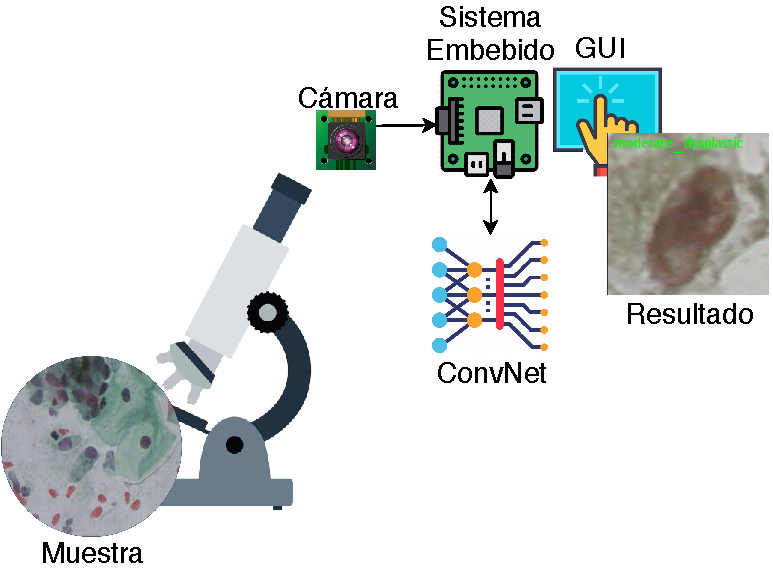
\includegraphics[width=0.6\textwidth]{capitulo_generalidades/diagrama_sistema}
    \caption{Diagrama del diseño conceptual}\label{fig:diagrama_sistema}
\end{figure}